\documentclass[11pt, letterpaper]{article}

\usepackage{amsmath}
\usepackage{amssymb}
\usepackage{amsthm}
\usepackage{geometry}
\usepackage{tikz}
\usetikzlibrary{arrows.meta, positioning, shapes, backgrounds}
\usepackage{mathrsfs}
\usepackage{mathtools}
\usepackage{hyperref}

\geometry{margin=1in}

\title{Homework 2: Conditional Probability \& Independence}
\author{Tashfeen Omran}
\date{September 2026}

\newtheorem{theorem}{Theorem}[section]
\newtheorem{lemma}[theorem]{Lemma}
\newtheorem{proposition}[theorem]{Proposition}
\newtheorem{corollary}[theorem]{Corollary}
\theoremstyle{definition}
\newtheorem{definition}{Definition}[section]
\newtheorem{problem}{Problem}
\newtheorem{axiom}{Axiom}[section]

\begin{document}

\maketitle
\tableofcontents
\newpage

\section{Part 1: Comprehensive Introduction, Context, and Prerequisites}

\subsection{Conceptual Introduction \& Historical Context}
The study of probability historically relied on physical intuition---coin flips, dice rolls, and card games. However, in the early 20th century, mathematicians faced a foundational crisis: paradoxes (such as the Bertrand Paradox) demonstrated that relying on geometric intuition without rigorous definitions leads to contradictory probabilities. In 1933, Andrey Kolmogorov resolved this by formalizing probability using measure theory, publishing \textit{Grundbegriffe der Wahrscheinlichkeitsrechnung} (Foundations of the Theory of Probability). 

Kolmogorov mapped the concept of ``events'' to sets, and ``probability'' to a mathematical measure. This profound abstraction unified probability with Lebesgue integration and real analysis, allowing it to serve as the bedrock for modern Artificial Intelligence, Machine Learning, and Quantitative Finance.

\subsection{Core Concepts \& Axioms}
In abstract probability, we define a \textbf{Probability Space} as a mathematical triplet $(\Omega, \mathscr{F}, \mathbb{P})$:
\begin{enumerate}
    \item \textbf{Sample Space ($\Omega$):} The set of all possible fundamental outcomes of a stochastic process.
    \item \textbf{Sigma-Algebra ($\mathscr{F}$):} A collection of subsets of $\Omega$ representing all permissible ``events'' that can be measured. It must contain $\Omega$, be closed under complementation, and closed under countable unions.
    \item \textbf{Probability Measure ($\mathbb{P}$):} A set function $\mathbb{P} : \mathscr{F} \to [0, 1]$ mapping events to numbers.
\end{enumerate}

The measure $\mathbb{P}$ must satisfy \textbf{Kolmogorov's Axioms}:
\begin{axiom}[Non-negativity]
For any event $A \in \mathscr{F}$, $\mathbb{P}(A) \geq 0$.
\end{axiom}
\begin{axiom}[Unit Measure]
$\mathbb{P}(\Omega) = 1$.
\end{axiom}
\begin{axiom}[Countable Additivity]
If $A_1, A_2, \dots \in \mathscr{F}$ are mutually exclusive (disjoint) events, then $\mathbb{P} \left( \bigcup_{i=1}^\infty A_i \right) = \sum_{i=1}^\infty \mathbb{P}(A_i)$.
\end{axiom}

\subsection{Intuition: Independence and Conditioning}
Conditional probability fundamentally restricts our universe from $\Omega$ down to a known event $B$. The new probability of $A$, given that $B$ has occurred, is the measure of the overlap between $A$ and $B$, scaled by the measure of $B$ to ensure the new universe integrates to $1$. Two events are \textbf{independent} if knowing that $B$ occurred provides no informational update regarding the likelihood of $A$. 

\subsection{Key Theorems \& Lemmas}
\begin{theorem}[Definition of Conditional Probability]
For events $A, B \in \mathscr{F}$ with $\mathbb{P}(B) > 0$, the conditional probability is:
\[ \mathbb{P}(A|B) = \frac{\mathbb{P}(A \cap B)}{\mathbb{P}(B)} \]
\end{theorem}
\begin{theorem}[Definition of Independence]
Events $A$ and $B$ are independent if and only if:
\[ \mathbb{P}(A \cap B) = \mathbb{P}(A)\mathbb{P}(B) \]
\end{theorem}
\begin{theorem}[Additive Law]
For any two events $A, B \in \mathscr{F}$:
\[ \mathbb{P}(A \cup B) = \mathbb{P}(A) + \mathbb{P}(B) - \mathbb{P}(A \cap B) \]
\end{theorem}

\subsection{Prerequisites}
To fully master this module, the reader must be proficient in:
\begin{itemize}
    \item \textbf{Set Theory:} Intersections ($\cap$), unions ($\cup$), complements ($\overline{A}$), and De Morgan's Laws.
    \item \textbf{Proof Techniques:} Direct algebraic deduction, proof by induction, and combinatorial proofs.
    \item \textbf{Combinatorics:} Binomial coefficients ($\binom{n}{k}$) and the Binomial Theorem.
\end{itemize}

\newpage
\section{Part 2: Detailed Homework Solutions (Rigorous Proofs)}
\textit{Note: This section strictly resolves the theoretical and proof-based subset of the assigned text, omitting pure arithmetic exercises to maintain the document's advanced abstract mathematical focus.}

\subsection{Combinatorics and Set Partitions}

\begin{problem}[Exercise 2.68]
Show that for any integer $n \geq 1$:
(a) $\binom{n}{0} = 1$, (b) $\binom{n}{n} = 1$, (c) $\binom{n}{r} = \binom{n}{n-r}$, (d) $\sum_{i=0}^n \binom{n}{i} = 2^n$.
\end{problem}
\begin{proof}
\textbf{Proof Technique:} Direct algebraic proof using factorial definitions and the Binomial Theorem.
By definition, the binomial coefficient is $\binom{n}{k} = \frac{n!}{k!(n-k)!}$.
\begin{itemize}
    \item[\textbf{(a)}] Setting $k = 0$:
    \[ \binom{n}{0} = \frac{n!}{0!(n-0)!} = \frac{n!}{1 \cdot n!} = 1 \]
    \textit{Interpretation:} There is exactly $1$ way to choose a null subset from $n$ items.
    
    \item[\textbf{(b)}] Setting $k = n$:
    \[ \binom{n}{n} = \frac{n!}{n!(n-n)!} = \frac{n!}{n!0!} = \frac{n!}{n! \cdot 1} = 1 \]
    \textit{Interpretation:} There is exactly $1$ way to select all items.
    
    \item[\textbf{(c)}] Let $r$ be an integer such that $0 \leq r \leq n$. Using the factorial definition:
    \[ \binom{n}{r} = \frac{n!}{r!(n-r)!} \]
    Rearranging the factors in the denominator yields:
    \[ \frac{n!}{(n-r)!r!} = \frac{n!}{(n-r)!(n - (n-r))!} = \binom{n}{n-r} \]
    \textit{Interpretation:} Choosing $r$ items to include is mathematically identical to choosing $n-r$ items to exclude.
    
    \item[\textbf{(d)}] Consider the formal Binomial Expansion of $(x+y)^n$:
    \[ (x+y)^n = \sum_{i=0}^n \binom{n}{i} x^i y^{n-i} \]
    Let $x = 1$ and $y = 1$. Substituting these values into the expansion gives:
    \[ (1+1)^n = \sum_{i=0}^n \binom{n}{i} (1)^i (1)^{n-i} \]
    Since $1$ raised to any power is $1$, this simplifies directly to:
    \[ 2^n = \sum_{i=0}^n \binom{n}{i} \]
    \textit{Interpretation:} The sum of the sizes of all possible subsets of a set of size $n$ equals the cardinality of the power set, $2^n$.
\end{itemize}
\end{proof}

\vspace{0.5cm}

\begin{problem}[Exercise 2.69]
Prove that $\binom{n+1}{r} = \binom{n}{r} + \binom{n}{r-1}$.
\end{problem}
\begin{proof}
\textbf{Proof Technique:} Direct algebraic manipulation.
Begin with the definitions of the two terms on the right-hand side:
\[ \binom{n}{r} + \binom{n}{r-1} = \frac{n!}{r!(n-r)!} + \frac{n!}{(r-1)!(n-(r-1))!} \]
Simplify the second denominator to $(r-1)!(n-r+1)!$:
\[ = \frac{n!}{r!(n-r)!} + \frac{n!}{(r-1)!(n-r+1)!} \]
To add these fractions, we must find a common denominator. The lowest common denominator is $r!(n-r+1)!$. We multiply the numerator and denominator of the first fraction by $(n-r+1)$, and the second by $r$:
\[ = \frac{n!(n-r+1)}{r!(n-r)!(n-r+1)} + \frac{n!(r)}{(r-1)!(r)(n-r+1)!} \]
Combine the factorial terms in the denominators ($k! = k \cdot (k-1)!$):
\[ = \frac{n!(n-r+1)}{r!(n-r+1)!} + \frac{n!(r)}{r!(n-r+1)!} \]
Combine the numerators over the common denominator:
\[ = \frac{n!(n-r+1) + n!(r)}{r!(n-r+1)!} \]
Factor out the common term $n!$ in the numerator:
\[ = \frac{n! [ (n-r+1) + r ]}{r!(n-r+1)!} \]
Simplify the bracketed term: $(n - r + 1 + r) = (n + 1)$:
\[ = \frac{n!(n+1)}{r!(n-r+1)!} \]
Recognize that $n!(n+1) = (n+1)!$ and rewrite the denominator:
\[ = \frac{(n+1)!}{r!((n+1)-r)!} = \binom{n+1}{r} \]
This completes the proof. $\blacksquare$
\end{proof}

\vspace{0.5cm}

\begin{problem}[Exercise 2.70]
Consider the situation where $n$ items are to be partitioned into $k < n$ distinct subsets. Prove that the total number of distinct partitions equals $k^n$.
\end{problem}
\begin{proof}
\textbf{Proof Technique:} Combinatorial proof utilizing the Multinomial Theorem.
By definition, a partition maps each of the $n$ distinct items to exactly one of the $k$ distinct subsets. Let the sizes of the $k$ subsets be $n_1, n_2, \dots, n_k$, such that $\sum_{i=1}^k n_i = n$.
The number of ways to partition the $n$ items into specific subset sizes $n_1, \dots, n_k$ is given by the multinomial coefficient:
\[ \binom{n}{n_1, n_2, \dots, n_k} = \frac{n!}{n_1! n_2! \dots n_k!} \]
To find the total number of distinct partitions, we sum over all valid non-negative integer configurations of $n_1, \dots, n_k$ that sum to $n$:
\[ \text{Total Partitions} = \sum_{n_1+\dots+n_k=n} \binom{n}{n_1, n_2, \dots, n_k} \]
By the Multinomial Theorem, for any real numbers $x_1, \dots, x_k$:
\[ (x_1 + x_2 + \dots + x_k)^n = \sum_{n_1+\dots+n_k=n} \binom{n}{n_1, \dots, n_k} x_1^{n_1} x_2^{n_2} \dots x_k^{n_k} \]
Let $x_i = 1$ for all $i = 1, \dots, k$. Substituting these values:
\[ (1 + 1 + \dots + 1)^n = \sum_{n_1+\dots+n_k=n} \binom{n}{n_1, \dots, n_k} 1^{n_1} \dots 1^{n_k} \]
\[ k^n = \sum_{n_1+\dots+n_k=n} \binom{n}{n_1, \dots, n_k} \]
Hence, the total number of distinct partitions is $k^n$. Intuitively, this represents $k$ independent choices for each of the $n$ items. $\blacksquare$
\end{proof}

\subsection{Foundations of Independence and Conditional Probability}

\begin{problem}[Exercise 2.78]
Show that if $P(A|B) = P(A)$, then $P(B|A) = P(B)$ and $P(A \cap B) = P(A)P(B)$.
\end{problem}
\begin{proof}
\textbf{Proof Technique:} Direct algebraic deduction.
Assume $P(B) > 0$ and $P(A) > 0$. We are given:
\[ P(A|B) = P(A) \]
By the definition of conditional probability:
\[ \frac{P(A \cap B)}{P(B)} = P(A) \]
Multiply both sides by $P(B)$:
\[ P(A \cap B) = P(A)P(B) \]
This proves the second required equality. Now, to prove the first equality, consider $P(B|A)$:
\[ P(B|A) = \frac{P(B \cap A)}{P(A)} \]
Since set intersection is commutative ($B \cap A = A \cap B$), we substitute $P(A \cap B)$ with $P(A)P(B)$:
\[ P(B|A) = \frac{P(A)P(B)}{P(A)} \]
Cancel $P(A)$ (valid since $P(A) > 0$):
\[ P(B|A) = P(B) \]
This demonstrates that all three conditions of independence are logically equivalent. $\blacksquare$
\end{proof}

\vspace{0.5cm}

\begin{problem}[Exercise 2.79]
If $P(A) > 0, P(B) > 0$, and $P(A) < P(A|B)$, show that $P(B) < P(B|A)$.
\end{problem}
\begin{proof}
\textbf{Proof Technique:} Strict inequality manipulation.
We are given:
\[ P(A) < P(A|B) \]
Apply the definition of conditional probability:
\[ P(A) < \frac{P(A \cap B)}{P(B)} \]
Since $P(B) > 0$, we can safely multiply both sides by $P(B)$ without flipping the inequality:
\[ P(A)P(B) < P(A \cap B) \]
Since $P(A) > 0$, we can divide both sides by $P(A)$:
\[ P(B) < \frac{P(A \cap B)}{P(A)} \]
By definition, the right side is $P(B|A)$. Thus:
\[ P(B) < P(B|A) \]
This confirms the symmetry of positive dependence. $\blacksquare$
\end{proof}

\vspace{0.5cm}

\begin{problem}[Exercise 2.80]
Suppose $A \subset B$ and $P(A) > 0$, $P(B) > 0$. Are $A$ and $B$ independent? Prove your answer.
\end{problem}
\begin{proof}
\textbf{Proof Technique:} Proof by Contradiction / Logical equivalence.
If $A \subset B$, then every element in $A$ is also in $B$. Therefore, their intersection is exactly $A$:
\[ A \cap B = A \implies P(A \cap B) = P(A) \]
For events $A$ and $B$ to be independent, we must have:
\[ P(A \cap B) = P(A)P(B) \]
Substituting $P(A \cap B)$ with $P(A)$:
\[ P(A) = P(A)P(B) \]
Since $P(A) > 0$, we divide both sides by $P(A)$:
\[ 1 = P(B) \]
Therefore, $A$ and $B$ are independent \textit{if and only if} $P(B) = 1$. Since the problem only states $P(B) > 0$, we cannot guarantee $P(B) = 1$. In general, a proper subset relationship heavily violates independence, making the events dependent. $\blacksquare$
\end{proof}

\vspace{0.5cm}

\begin{problem}[Exercise 2.81 \& 2.83]
\textbf{Part 1 (2.81):} Suppose $A$ and $B$ are mutually exclusive events, $P(A)>0, P(B)>0$. Are they independent?
\textbf{Part 2 (2.83):} If $A, B$ are mutually exclusive and $P(B)>0$, show that $P(A | A \cup B) = \frac{P(A)}{P(A) + P(B)}$.
\end{problem}
\begin{proof}
\textbf{Part 1 (Independence):}
By definition, mutually exclusive events cannot occur simultaneously. Hence, their intersection is the null set ($\emptyset$):
\[ A \cap B = \emptyset \implies P(A \cap B) = 0 \]
If they were independent, $P(A \cap B) = P(A)P(B)$. However, because $P(A)>0$ and $P(B)>0$, their product is strictly positive:
\[ P(A)P(B) > 0 \]
Since $0 \neq P(A)P(B)$, the events are strongly dependent. (If one occurs, the other cannot occur, which is the ultimate form of dependence). 

\textbf{Part 2 (Conditional Probability):}
By the definition of conditional probability:
\[ P(A | A \cup B) = \frac{P(A \cap (A \cup B))}{P(A \cup B)} \]
Because $A$ is a subset of $A \cup B$, the intersection is simply $A$: $A \cap (A \cup B) = A$.
\[ P(A | A \cup B) = \frac{P(A)}{P(A \cup B)} \]
By the Axiom of Additivity for mutually exclusive events, $P(A \cup B) = P(A) + P(B)$. Therefore:
\[ P(A | A \cup B) = \frac{P(A)}{P(A) + P(B)} \]
$\blacksquare$
\end{proof}

\vspace{0.5cm}

\begin{problem}[Exercise 2.84]
If $A_1, A_2, A_3$ are three events such that $P(A_1 \cap A_2) = P(A_1 \cap A_3) \neq 0$ but $P(A_2 \cap A_3) = 0$. Show that $P(\text{at least one } A_i) = P(A_1) + P(A_2) + P(A_3) - 2P(A_1 \cap A_2)$.
\end{problem}
\begin{proof}
\textbf{Proof Technique:} Inclusion-Exclusion Principle.
The event ``at least one $A_i$ occurs'' is represented by the union $A_1 \cup A_2 \cup A_3$. By the general additive law (Inclusion-Exclusion Principle):
\[ P(A_1 \cup A_2 \cup A_3) = \sum_{i=1}^3 P(A_i) - P(A_1 \cap A_2) - P(A_1 \cap A_3) - P(A_2 \cap A_3) + P(A_1 \cap A_2 \cap A_3) \]
We are given $P(A_2 \cap A_3) = 0$. Since the triple intersection $(A_1 \cap A_2 \cap A_3) \subseteq (A_2 \cap A_3)$, monotonicity of measures implies:
\[ P(A_1 \cap A_2 \cap A_3) \leq P(A_2 \cap A_3) = 0 \implies P(A_1 \cap A_2 \cap A_3) = 0 \]
Substitute these zeros into the equation:
\[ P(A_1 \cup A_2 \cup A_3) = P(A_1) + P(A_2) + P(A_3) - P(A_1 \cap A_2) - P(A_1 \cap A_3) - 0 + 0 \]
We are also given $P(A_1 \cap A_3) = P(A_1 \cap A_2)$. Substitute this term:
\[ = P(A_1) + P(A_2) + P(A_3) - P(A_1 \cap A_2) - P(A_1 \cap A_2) \]
\[ = P(A_1) + P(A_2) + P(A_3) - 2P(A_1 \cap A_2) \]
$\blacksquare$
\end{proof}

\vspace{0.5cm}

\begin{problem}[Exercise 2.85]
If $A$ and $B$ are independent events, show that $A$ and $\overline{B}$ are independent. Then, show that $\overline{A}$ and $\overline{B}$ are independent.
\end{problem}
\begin{proof}
\textbf{Proof Technique:} Set Partitioning and De Morgan's Laws.
\textbf{Part 1:} We must show $P(A \cap \overline{B}) = P(A)P(\overline{B})$.
By the Law of Total Probability, the set $A$ can be partitioned into its intersection with $B$ and its intersection with $\overline{B}$:
\[ P(A) = P(A \cap B) + P(A \cap \overline{B}) \]
Rearranging for $P(A \cap \overline{B})$:
\[ P(A \cap \overline{B}) = P(A) - P(A \cap B) \]
Because $A$ and $B$ are independent, substitute $P(A \cap B) = P(A)P(B)$:
\[ P(A \cap \overline{B}) = P(A) - P(A)P(B) \]
Factor out $P(A)$:
\[ P(A \cap \overline{B}) = P(A)(1 - P(B)) \]
Since $(1 - P(B)) = P(\overline{B})$:
\[ P(A \cap \overline{B}) = P(A)P(\overline{B}) \]
Thus, $A$ and $\overline{B}$ are independent.

\textbf{Part 2:} We must show $P(\overline{A} \cap \overline{B}) = P(\overline{A})P(\overline{B})$.
By De Morgan's Law, $\overline{A} \cap \overline{B} = \overline{A \cup B}$. Therefore:
\[ P(\overline{A} \cap \overline{B}) = 1 - P(A \cup B) \]
Apply the additive law for $P(A \cup B)$:
\[ = 1 - [P(A) + P(B) - P(A \cap B)] \]
Because $A$ and $B$ are independent:
\[ = 1 - P(A) - P(B) + P(A)P(B) \]
Factor this algebraic expression by grouping:
\[ = (1 - P(A)) - P(B)(1 - P(A)) \]
\[ = (1 - P(A))(1 - P(B)) \]
Substitute the definitions of the complements:
\[ = P(\overline{A})P(\overline{B}) \]
$\blacksquare$
\end{proof}

\vspace{0.5cm}

\begin{problem}[Exercise 2.100]
Show that Theorem 2.6, the additive law, holds for conditional probabilities. Prove that $P(A \cup B | C) = P(A|C) + P(B|C) - P(A \cap B | C)$.
\end{problem}
\begin{proof}
\textbf{Proof Technique:} Set Theory Distributivity.
Start with the definition of conditional probability:
\[ P(A \cup B | C) = \frac{P((A \cup B) \cap C)}{P(C)} \]
By the distributive law of sets, $(A \cup B) \cap C = (A \cap C) \cup (B \cap C)$. Substitute this back:
\[ = \frac{P((A \cap C) \cup (B \cap C))}{P(C)} \]
Apply the standard additive law in the numerator:
\[ P((A \cap C) \cup (B \cap C)) = P(A \cap C) + P(B \cap C) - P((A \cap C) \cap (B \cap C)) \]
Notice that $(A \cap C) \cap (B \cap C) = A \cap B \cap C$. Therefore, the numerator is:
\[ = \frac{P(A \cap C) + P(B \cap C) - P(A \cap B \cap C)}{P(C)} \]
Separate the fractions:
\[ = \frac{P(A \cap C)}{P(C)} + \frac{P(B \cap C)}{P(C)} - \frac{P(A \cap B \cap C)}{P(C)} \]
Apply the definition of conditional probability to each term independently:
\[ = P(A|C) + P(B|C) - P(A \cap B | C) \]
$\blacksquare$
\end{proof}

\vspace{0.5cm}

\begin{problem}[Exercise 2.104]
Prove that $P(A \cap B) \geq 1 - P(\overline{A}) - P(\overline{B})$. (Simplified Bonferroni Inequality).
\end{problem}
\begin{proof}
\textbf{Proof Technique:} Measure bounds and Complements.
Begin with the rearranged Additive Law of Probability:
\[ P(A \cap B) = P(A) + P(B) - P(A \cup B) \]
By Kolmogorov's second axiom, probability measures are bounded by $1$. Therefore, $P(A \cup B) \leq 1$. Subtracting a smaller or equal number yields a larger or equal result, hence:
\[ -P(A \cup B) \geq -1 \]
Substitute this inequality into the additive law equation:
\[ P(A \cap B) \geq P(A) + P(B) - 1 \]
Using the complement rule, substitute $P(A) = 1 - P(\overline{A})$ and $P(B) = 1 - P(\overline{B})$:
\[ P(A \cap B) \geq (1 - P(\overline{A})) + (1 - P(\overline{B})) - 1 \]
Simplify the algebraic terms:
\[ P(A \cap B) \geq 2 - 1 - P(\overline{A}) - P(\overline{B}) \]
\[ P(A \cap B) \geq 1 - P(\overline{A}) - P(\overline{B}) \]
This bound is critical when $A$ and $B$ are highly probable events. $\blacksquare$
\end{proof}

\vspace{0.5cm}

\begin{problem}[Exercise 2.119]
Two balanced dice are tossed repeatedly. What is the probability that we obtain a sum of 3 before a sum of 7?
\end{problem}
\begin{proof}
\textbf{Proof Technique:} Infinite Geometric Series / Markov State Transition.
Let $\Omega$ represent the sample space of tossing two dice, with cardinality $36$.
Let $E$ be the event of rolling a 3. Outcomes are $(1,2), (2,1)$. Thus, $P(E) = \frac{2}{36}$.
Let $F$ be the event of rolling a 7. Outcomes are $(1,6), (2,5), (3,4), (4,3), (5,2), (6,1)$. Thus, $P(F) = \frac{6}{36}$.
Let $G$ be the event of rolling neither. $P(G) = 1 - P(E) - P(F) = 1 - \frac{8}{36} = \frac{28}{36}$.

We want the probability of $E$ occurring before $F$. This happens if we roll $E$ on the 1st turn, OR roll $G$ then $E$, OR roll $G, G,$ then $E$, and so on.
\[ \mathbb{P}(\text{3 before 7}) = P(E) + P(G)P(E) + P(G)^2P(E) + \dots = \sum_{k=0}^\infty P(G)^k P(E) \]
This is a convergent geometric series with ratio $|P(G)| < 1$. The sum evaluates to:
\[ = \frac{P(E)}{1 - P(G)} \]
Substitute $1 - P(G) = P(E) + P(F)$:
\[ = \frac{P(E)}{P(E) + P(F)} \]
\[ = \frac{2/36}{2/36 + 6/36} = \frac{2}{8} = \frac{1}{4} \]
Therefore, the probability is strictly $0.25$. $\blacksquare$
\end{proof}

\newpage
\section{Part 3: In-Depth Analysis of Problems and Techniques}

\subsection{A) Problem Types and Logical Strategies}
Reviewing the solved exercises, the mathematical framework can be mapped to three overarching paradigms:
\begin{enumerate}
    \item \textbf{Existence/Uniqueness and Combinatorial Arguments (e.g., 2.68, 2.70):} These problems rely on defining a mapping between spaces. The core strategy is to interpret numerical coefficients as discrete choice paradigms, utilizing the Multinomial Theorem as a continuous function proxy to bypass recursive counting limits.
    \item \textbf{Measure Inequalities (e.g., 2.104):} Probability is a bounded measure ($[0,1]$). The overarching strategy to find lower limits of intersection (Bonferroni) involves forcing the union to its supreme limit (1).
    \item \textbf{Stochastic State Transitions (e.g., 2.119):} Rather than evaluating a static probability, these models require infinite geometric summations or conditioning on a non-absorbing state. The strategy is to filter out the irrelevant state transitions (event $G$) and condition exclusively on the absorbing states ($E$ and $F$).
\end{enumerate}

\subsection{B) Key Analytical and Logical Manipulations}
\begin{itemize}
    \item \textbf{De Morgan's Laws (Exercise 2.85):} The manipulation $\overline{A} \cap \overline{B} = \overline{A \cup B}$ is not merely algebraic; it maps a restrictive intersection space into a broad union complement, allowing the additive law to be triggered. 
    \item \textbf{Law of Total Probability Partitioning:} Breaking $A$ into $(A \cap B) \cup (A \cap \overline{B})$ allows us to isolate variables. This is the cornerstone of Bayesian updating---you marginalize out the latent variable $B$.
    \item \textbf{The Absorbing State "Cheat":} In infinite dice-rolling (2.119), evaluating $\frac{P(E)}{P(E) + P(F)}$ bypasses infinite series limits by directly normalizing the sample space to only those events that terminate the experiment.
\end{itemize}

\section{Part 4: "Cheatsheet", Visuals, and Tips for Success}

\subsection{Measure-Theoretic Venn Representation}
Below is a rigorous geometric visualization of conditional probability spaces.

\begin{center}
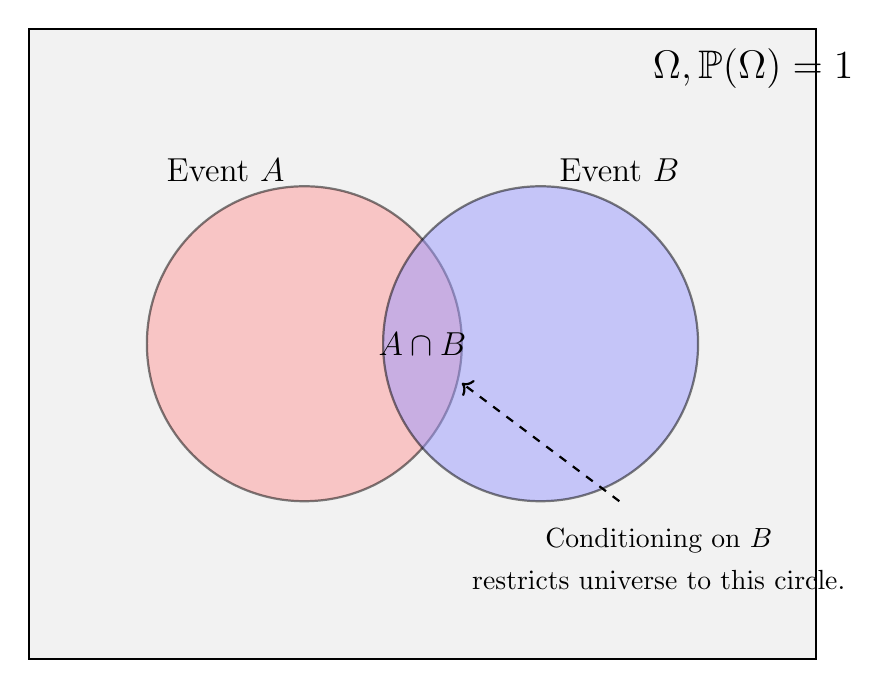
\begin{tikzpicture}[thick, set/.style={circle, minimum size=4cm, draw=black, fill=blue!10, opacity=0.5}]
    % Outer box (Omega)
    \draw[fill=gray!10] (-5,-4) rectangle (5,4);
    \node at (4.2, 3.5) {\Large $\Omega, \mathbb{P}(\Omega)=1$};
    
    % Sets A and B
    \node[set, fill=red!40] (A) at (-1.5,0) {};
    \node[set, fill=blue!40] (B) at (1.5,0) {};
    
    % Labels
    \node at (-2.5, 2.2) {\large Event $A$};
    \node at (2.5, 2.2) {\large Event $B$};
    
    \node at (0, 0) {\large $A \cap B$};
    
    % Arrows for Conditional Prob
    \draw[->, thick, dashed] (2.5, -2) -- (0.5, -0.5);
    \node at (3, -2.5) {Conditioning on $B$};
    \node at (3, -3) {restricts universe to this circle.};
\end{tikzpicture}
\end{center}

\subsection{Heuristics \& "Cheats"}
\begin{itemize}
    \item \textbf{The Independence Check:} If you see $A \subset B$, they are almost certainly dependent unless $P(B) = 1$. Subset structure forces deterministic linkage.
    \item \textbf{Complement Shortcut:} Anytime a problem asks for ``at least one'', immediately compute $1 - \mathbb{P}(\text{none})$. This swaps a massive inclusion-exclusion calculation for a single intersection.
\end{itemize}

\subsection{Pitfalls \& Fallacies}
\begin{itemize}
    \item \textbf{Mutually Exclusive vs. Independent Fallacy:} Assuming that because events do not overlap, they don't affect each other. This is fatal. If they don't overlap, the occurrence of one guarantees the non-occurrence of the other. They are maximally dependent.
    \item \textbf{Conditioning on a Complement:} A common algebraic error is assuming $P(A|B) + P(A|\overline{B}) = 1$. The true axiom is $P(A|B) + P(\overline{A}|B) = 1$. You must sum over the target variable, not the conditioned variable.
\end{itemize}

\newpage
\section{Part 5: Conceptual Synthesis and The "Big Picture"}

\subsection{A) Thematic Connections}
The core theme of this chapter is \textbf{utilizing set-theoretic abstractions to govern uncertainty}. By bridging Boolean algebra (unions, intersections) with measure theory (addition, limits), we establish a consistent, paradox-free engine for processing information. When we "condition" on $B$, we are functionally calculating the Radon-Nikodym derivative of the measure of $A$ with respect to the restricted subspace $B$.

\subsection{B) Forward and Backward Links}
Backwardly, this module completes the bridge from combinatorial counting sets into normalized continuous parameters $[0,1]$. Forwardly, understanding $\sigma$-algebras and independence is the exact prerequisite for defining \textbf{Filtrations} ($\mathscr{F}_t$), which represent the "history" of information in advanced Stochastic Calculus. Without the conditional probability structures proved in 2.100, we could not define Martingales, which are the backbone of algorithmic trading and deep reinforcement learning.

\section{Part 6: Abstract Real-World Modeling (AI, ML, \& Quant Finance)}

\subsection{A) Concrete Scenarios}
\begin{itemize}
    \item \textbf{Bayesian Neural Networks (AI):} Weights are treated not as scalars, but as probability distributions. The network relies heavily on independence identities (Exercise 2.85) to establish the Mean-Field Variational inference parameters.
    \item \textbf{Algorithmic Trading \& Default Contagion (Quant Finance):} When pricing synthetic Collateralized Debt Obligations (CDOs), the probability of Company A defaulting is highly dependent on whether Company B defaults. We use copulas and the Bonferroni inequalities (Exercise 2.104) to bound the tail-risk of joint failures.
\end{itemize}

\subsection{B) Model Problem Setup: Stochastic Calculus \& Risk Neutral Pricing}
In quantitative finance, the theoretical concepts from this homework are explicitly formulated as follows. Let $(\Omega, \mathscr{F}, \{\mathscr{F}_t\}_{t \geq 0}, \mathbb{P})$ be a filtered probability space. The $\sigma$-algebra $\mathscr{F}_t$ represents all market information available up to time $t$.

An asset price $X_t$ is modeled via the Stochastic Differential Equation (SDE) using Itô's Lemma:
\[ dX_t = \mu X_t \, dt + \sigma X_t \, dW_t \]
where $W_t$ is a standard Brownian motion. The fundamental theorem of asset pricing states that the fair price of a derivative $V(X_T)$ at time $t$ is its conditional expectation under a risk-neutral measure $\mathbb{Q}$:
\[ V_t = \mathbb{E}^{\mathbb{Q}}[e^{-r(T-t)} V(X_T) \mid \mathscr{F}_t] \]
This conditional expectation is the continuous-measure analogue of the discrete conditional probability $\mathbb{P}(A|B)$ you solved in Exercise 2.78. The information $\mathscr{F}_t$ plays the exact role of event $B$. Mastering how intersecting information spaces behave is essential to correctly computing these multi-million dollar derivative prices.

\newpage
\section{Part 7: Common Variations and Untested Concepts}

A standard university sequence on advanced probability usually includes infinite sequence limits, which were absent from the provided snapshot. 

\begin{theorem}[The Borel-Cantelli Lemma]
Let $\{A_n\}_{n=1}^\infty$ be a sequence of events in $\mathscr{F}$. If the sum of their probabilities converges, i.e., $\sum_{n=1}^\infty \mathbb{P}(A_n) < \infty$, then the probability that infinitely many of them occur is zero:
\[ \mathbb{P} \left( \limsup_{n \to \infty} A_n \right) = 0 \]
\end{theorem}
\begin{proof}
By definition, the limit superior of sets is $\limsup_{n \to \infty} A_n = \bigcap_{N=1}^\infty \bigcup_{n=N}^\infty A_n$.
Using the property of nested sets and Kolmogorov's axioms:
\[ \mathbb{P} \left( \bigcap_{N=1}^\infty \bigcup_{n=N}^\infty A_n \right) \leq \mathbb{P} \left( \bigcup_{n=N}^\infty A_n \right) \text{ for any } N \]
By Boole's inequality (subadditivity):
\[ \mathbb{P} \left( \bigcup_{n=N}^\infty A_n \right) \leq \sum_{n=N}^\infty \mathbb{P}(A_n) \]
Because the infinite series $\sum \mathbb{P}(A_n)$ converges, its tail sum must approach $0$ as $N \to \infty$. Thus, the probability is bounded by $0$. $\blacksquare$
\end{proof}

\section{Part 8: Advanced Diagnostic Testing: "Find the Flaw"}

Below are 5 advanced logic problems. Each contains a mathematically convincing step-by-step proof that holds a singular, catastrophic logical flaw. Act as the grader and find the errors. (Solutions provided at the end).

\begin{problem}
\textbf{The Pairwise Trap.}
Let $\Omega = \{1, 2, 3, 4\}$ with uniform probability. Let $A = \{1,2\}, B = \{1,3\}, C = \{1,4\}$. We check independence. $P(A) = 1/2$. $P(B) = 1/2$. $P(A \cap B) = P(\{1\}) = 1/4$. Since $1/4 = (1/2)(1/2)$, $A$ and $B$ are independent. Similarly, $A$ and $C$ are independent, and $B$ and $C$ are independent. Therefore, $A, B$, and $C$ are mutually independent events.
\end{problem}

\begin{problem}
\textbf{The Complement Shift.}
A medical test is given for a disease. We know that the probability of a patient having the disease given a positive test is $P(D|+) = 0.60$. Therefore, the probability that the patient has the disease given a negative test is $P(D|-) = 1 - 0.60 = 0.40$.
\end{problem}

\begin{problem}
\textbf{Zero-Probability Fallacy.}
Let $X$ be a random variable representing the exact time a train arrives between 12:00 and 1:00, uniformly distributed $X \sim \mathcal{U}(0,1)$. We want to find the probability that the train arrives in the first half hour, given it arrived exactly at 12:15. By definition:
\[ P(X \in [0, 0.5] \mid X = 0.25) = \frac{P(X \in [0, 0.5] \cap X = 0.25)}{P(X = 0.25)} \]
Since $X$ is continuous, $P(X = 0.25) = 0$. Thus we get $0 / 0$, which is mathematically undefined. Therefore, conditional probability does not exist for continuous events.
\end{problem}

\begin{problem}
\textbf{The Total Probability Misstep.}
An AI model predicts rain $A$ based on cloud cover $B$. We are given $P(A|B) = 0.8$ and $P(A|\overline{B}) = 0.1$. To find the unconditional probability of rain $P(A)$, we sum the conditionals: $P(A) = P(A|B) + P(A|\overline{B}) = 0.8 + 0.1 = 0.9$.
\end{problem}

\begin{problem}
\textbf{The Independence Disjoint Paradox.}
A standard die is rolled. Event $A$ is rolling a 2. Event $B$ is rolling a 3. Since it is impossible to roll a 2 and a 3 simultaneously, the events have absolutely nothing to do with each other. Therefore, because they are independent of each other physically, they are statistically independent.
\end{problem}

\vspace{0.5cm}
\hrule
\vspace{0.5cm}

\subsection{Solution Key for Flaw Diagnostics}
\begin{enumerate}
    \item \textbf{Flaw in 1:} The proof confuses \textit{pairwise} independence with \textit{mutual} independence. Mutual independence strictly requires $P(A \cap B \cap C) = P(A)P(B)P(C)$. Here, $P(A \cap B \cap C) = P(\{1\}) = 1/4$. However, $P(A)P(B)P(C) = 1/8$. Since $1/4 \neq 1/8$, they are not mutually independent.
    \item \textbf{Flaw in 2:} The complement rule applies to the conditioned event, not the conditioning space. The true identity is $P(\overline{D}|+) = 1 - 0.60 = 0.40$. You cannot deduce $P(D|-)$ without using Bayes' theorem and base rates.
    \item \textbf{Flaw in 3:} The fundamental flaw is using discrete probability formulas on measure-zero continuous sets without utilizing limits. In continuous measure theory (Radon-Nikodym), conditional probability on a point is handled via Regular Conditional Probabilities and limits. Evaluating to $0/0$ does not mean it is undefined; it requires L'Hôpital equivalent integration bounds.
    \item \textbf{Flaw in 4:} The proof attempts to use the Law of Total Probability but forgets to weight the conditional probabilities by the prior distribution of the states. The correct formulation must be $P(A) = P(A|B)P(B) + P(A|\overline{B})P(\overline{B})$.
    \item \textbf{Flaw in 5:} The colloquial definition of "independent" is falsely equated with the rigorous statistical definition. As proved in Homework Problem 2.81, mutually exclusive events with positive probabilities are strictly \textit{dependent}, because $P(A \cap B) = 0$, whereas $P(A)P(B) = (1/6)(1/6) \neq 0$.
\end{enumerate}

\end{document}